\documentclass[14pt]{extbook}
\usepackage{multicol, enumerate, enumitem, hyperref, color, soul, setspace, parskip, fancyhdr} %General Packages
\usepackage{amssymb, amsthm, amsmath, bbm, latexsym, units, mathtools} %Math Packages
\everymath{\displaystyle} %All math in Display Style
% Packages with additional options
\usepackage[headsep=0.5cm,headheight=12pt, left=1 in,right= 1 in,top= 1 in,bottom= 1 in]{geometry}
\usepackage[usenames,dvipsnames]{xcolor}
\usepackage{dashrule}  % Package to use the command below to create lines between items
\newcommand{\litem}[1]{\item#1\hspace*{-1cm}\rule{\textwidth}{0.4pt}}
\pagestyle{fancy}
\lhead{Progress Quiz 4}
\chead{}
\rhead{Version B}
\lfoot{6286-1986}
\cfoot{}
\rfoot{Fall 2020}
\begin{document}

\begin{enumerate}
\litem{
Describe the end behavior of the polynomial below.\[ f(x) = 9(x + 6)^{5}(x - 6)^{10}(x + 3)^{3}(x - 3)^{5} \]\begin{enumerate}[label=\Alph*.]
\begin{multicols}{2}\item 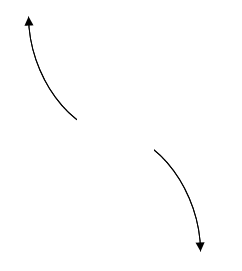
\includegraphics[width = 0.3\textwidth]{../Figures/polyEndBehaviorCopyAB.png}\item 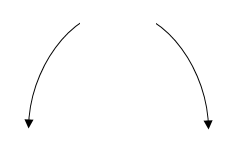
\includegraphics[width = 0.3\textwidth]{../Figures/polyEndBehaviorCopyBB.png}\item 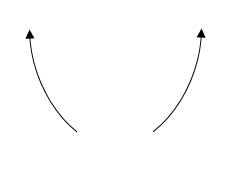
\includegraphics[width = 0.3\textwidth]{../Figures/polyEndBehaviorCopyCB.png}\item 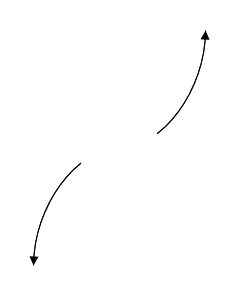
\includegraphics[width = 0.3\textwidth]{../Figures/polyEndBehaviorCopyDB.png}\end{multicols}\item None of the above.
\end{enumerate} }
\litem{
Construct the lowest-degree polynomial given the zeros below. Then, choose the intervals that contain the coefficients of the polynomial in the form $ax^3+bx^2+cx+d$.\[ 7, 6, \text{ and } \frac{-7}{4} \]\begin{enumerate}[label=\Alph*.]
\item \( a \in [-1, 5], b \in [-51, -40], c \in [74, 78], \text{ and } d \in [-295, -287] \)
\item \( a \in [-1, 5], b \in [43, 49], c \in [74, 78], \text{ and } d \in [-295, -287] \)
\item \( a \in [-1, 5], b \in [-51, -40], c \in [74, 78], \text{ and } d \in [287, 297] \)
\item \( a \in [-1, 5], b \in [58, 62], c \in [256, 261], \text{ and } d \in [287, 297] \)
\item \( a \in [-1, 5], b \in [11, 13], c \in [-164, -157], \text{ and } d \in [-295, -287] \)

\end{enumerate} }
\litem{
Construct the lowest-degree polynomial given the zeros below. Then, choose the intervals that contain the coefficients of the polynomial in the form $x^3+bx^2+cx+d$.\[ -4 + 2 i \text{ and } -3 \]\begin{enumerate}[label=\Alph*.]
\item \( b \in [-1, 7], c \in [-1, 4], \text{ and } d \in [-13, -3] \)
\item \( b \in [10, 18], c \in [41, 45], \text{ and } d \in [55, 73] \)
\item \( b \in [-11, -4], c \in [41, 45], \text{ and } d \in [-60, -58] \)
\item \( b \in [-1, 7], c \in [7, 13], \text{ and } d \in [8, 17] \)
\item \( \text{None of the above.} \)

\end{enumerate} }
\litem{
Describe the end behavior of the polynomial below.\[ f(x) = -8(x - 4)^{5}(x + 4)^{8}(x + 3)^{4}(x - 3)^{6} \]\begin{enumerate}[label=\Alph*.]
\begin{multicols}{2}\item 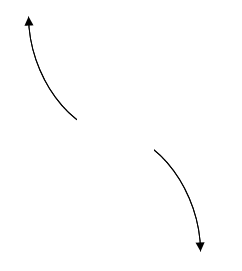
\includegraphics[width = 0.3\textwidth]{../Figures/polyEndBehaviorAB.png}\item 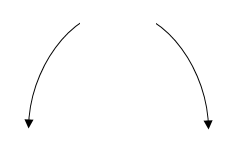
\includegraphics[width = 0.3\textwidth]{../Figures/polyEndBehaviorBB.png}\item 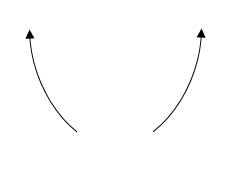
\includegraphics[width = 0.3\textwidth]{../Figures/polyEndBehaviorCB.png}\item 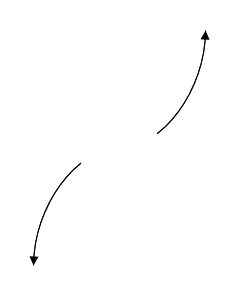
\includegraphics[width = 0.3\textwidth]{../Figures/polyEndBehaviorDB.png}\end{multicols}\item None of the above.
\end{enumerate} }
\litem{
Which of the following equations \textit{could} be of the graph presented below?
\begin{center}
    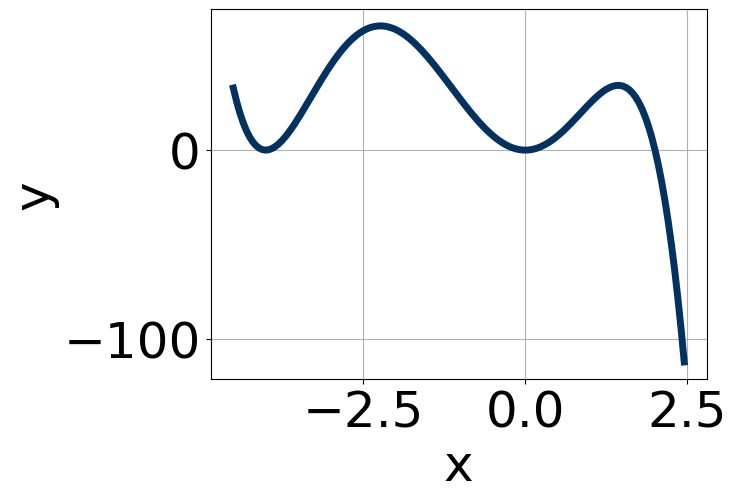
\includegraphics[width=0.5\textwidth]{../Figures/polyGraphToFunctionCopyB.png}
\end{center}
\begin{enumerate}[label=\Alph*.]
\item \( 13(x - 2)^{10} (x - 3)^{4} (x + 2)^{4} \)
\item \( 2(x - 2)^{8} (x - 3)^{10} (x + 2)^{7} \)
\item \( -8(x - 2)^{10} (x - 3)^{4} (x + 2)^{9} \)
\item \( -3(x - 2)^{4} (x - 3)^{5} (x + 2)^{9} \)
\item \( -16(x - 2)^{6} (x - 3)^{7} (x + 2)^{10} \)

\end{enumerate} }
\litem{
Which of the following equations \textit{could} be of the graph presented below?
\begin{center}
    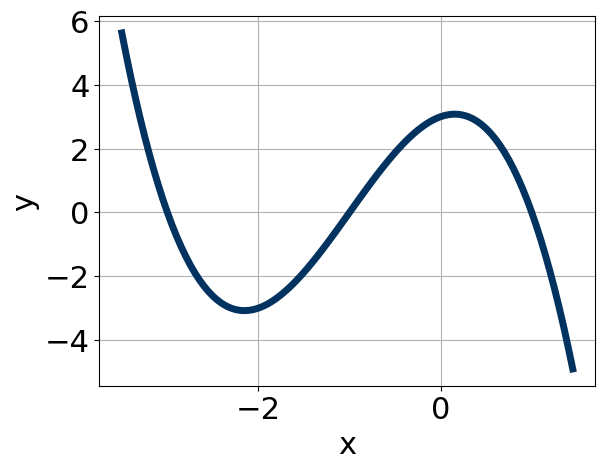
\includegraphics[width=0.5\textwidth]{../Figures/polyGraphToFunctionB.png}
\end{center}
\begin{enumerate}[label=\Alph*.]
\item \( 13x^{10} (x - 2)^{4} (x + 1)^{11} \)
\item \( -8x^{6} (x - 2)^{5} (x + 1)^{4} \)
\item \( -16x^{8} (x - 2)^{5} (x + 1)^{5} \)
\item \( 3x^{11} (x - 2)^{6} (x + 1)^{9} \)
\item \( 13x^{8} (x - 2)^{5} (x + 1)^{7} \)

\end{enumerate} }
\litem{
Construct the lowest-degree polynomial given the zeros below. Then, choose the intervals that contain the coefficients of the polynomial in the form $ax^3+bx^2+cx+d$.\[ \frac{-4}{5}, \frac{-2}{3}, \text{ and } 3 \]\begin{enumerate}[label=\Alph*.]
\item \( a \in [10, 22], b \in [-24, -20], c \in [-64, -57], \text{ and } d \in [-24, -18] \)
\item \( a \in [10, 22], b \in [-51, -42], c \in [-8, 5], \text{ and } d \in [22, 29] \)
\item \( a \in [10, 22], b \in [-70, -60], c \in [74, 80], \text{ and } d \in [-24, -18] \)
\item \( a \in [10, 22], b \in [-24, -20], c \in [-64, -57], \text{ and } d \in [22, 29] \)
\item \( a \in [10, 22], b \in [18, 27], c \in [-64, -57], \text{ and } d \in [22, 29] \)

\end{enumerate} }
\litem{
Describe the zero behavior of the zero $x = 9$ of the polynomial below.\[ f(x) = 7(x - 9)^{6}(x + 9)^{7}(x - 6)^{7}(x + 6)^{11} \]\begin{enumerate}[label=\Alph*.]
\begin{multicols}{2}\item 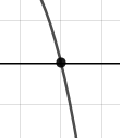
\includegraphics[width = 0.3\textwidth]{../Figures/polyZeroBehaviorCopyAB.png}\item 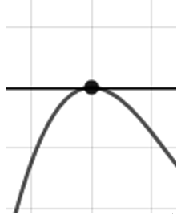
\includegraphics[width = 0.3\textwidth]{../Figures/polyZeroBehaviorCopyBB.png}\item 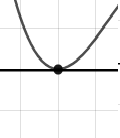
\includegraphics[width = 0.3\textwidth]{../Figures/polyZeroBehaviorCopyCB.png}\item 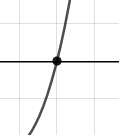
\includegraphics[width = 0.3\textwidth]{../Figures/polyZeroBehaviorCopyDB.png}\end{multicols}\item None of the above.
\end{enumerate} }
\litem{
Construct the lowest-degree polynomial given the zeros below. Then, choose the intervals that contain the coefficients of the polynomial in the form $x^3+bx^2+cx+d$.\[ -4 - 3 i \text{ and } -2 \]\begin{enumerate}[label=\Alph*.]
\item \( b \in [0, 7], c \in [3.09, 5.81], \text{ and } d \in [5.4, 7.3] \)
\item \( b \in [-10, -3], c \in [40.53, 42.29], \text{ and } d \in [-52, -49.7] \)
\item \( b \in [9, 16], c \in [40.53, 42.29], \text{ and } d \in [49, 50.4] \)
\item \( b \in [0, 7], c \in [5.46, 7.06], \text{ and } d \in [7, 11.7] \)
\item \( \text{None of the above.} \)

\end{enumerate} }
\litem{
Describe the zero behavior of the zero $x = 5$ of the polynomial below.\[ f(x) = 2(x + 5)^{3}(x - 5)^{8}(x + 7)^{9}(x - 7)^{10} \]\begin{enumerate}[label=\Alph*.]
\begin{multicols}{2}\item 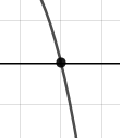
\includegraphics[width = 0.3\textwidth]{../Figures/polyZeroBehaviorAB.png}\item 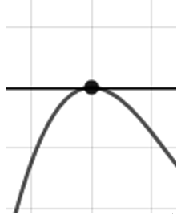
\includegraphics[width = 0.3\textwidth]{../Figures/polyZeroBehaviorBB.png}\item 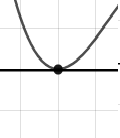
\includegraphics[width = 0.3\textwidth]{../Figures/polyZeroBehaviorCB.png}\item 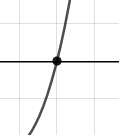
\includegraphics[width = 0.3\textwidth]{../Figures/polyZeroBehaviorDB.png}\end{multicols}\item None of the above.
\end{enumerate} }
\end{enumerate}

\end{document}